
%%
%% Template chap2.tex
%%

\chapter{Experiment 2: Learning with Thompson Sampling}
\label{cha:expt2}

Let us now turn our attention to active learning. In this chapter,
we investigate the 6 active learning heuristics described in section \ref{sec:heuristics}:
two uncertainty sampling heuristics (with either entropy or margin), two query
by bagging heuristics (with either margin or KL divergence), variance minimisation,
and classifier certainty. The goal is to see which ones can outperform
random sampling from the previous chapter. We then use Thompson sampling to see if
it can automatically filter out the bad heuristics and select the best one.


\section{Experimental Protocol}
\label{sec:protocol2}

Out of the four classifiers studied in Chapter \ref{cha:expt1}, only logistic regression
and RBF SVM provide reliable probability estimates. Random forests are able to predict
class probabilities by looking at the distribution of votes. However, we find in practice
that they are not stable (see Appendix for an example). With linear SVMs, the probability 
functionality has not been implemented in Scikit-learn. Thus we are only left
with two choices: logistic regression and RBF SVM.

For the unlabelled pool, we examine two cases. In one case, the pool is balanced, with
an equal number of objects in each class. This allows us to find out the maximum
performance of the heuristics in the best possible scenario. Of course, in real life,
the classes are not evenly distributed. Thus in the second case, we keep the original
class distribution and see if the performance would deteriorate in any way.

Given that there are two datasets, two choices of classifiers, and two ways to construct the
unlabelled pool, we need to conduct in total eight runs for each heuristic.
In each run, we do a stratified shuffle split of the training and test data with 10 trials.
The learning curves are then averaged out.

All heuristics require probability estimates. Thus we need to start with a partially trained
classifier. Initially, 50 random examples are chosen for training. Then at each step,
we select a random sample of 300 and use the heuristics to rank these candidates. The best
one is then put in our training
set. We keep doing this until a sample size of 300 is achieved. For the committee heuristics,
we use 11 members.

Finally we repeat the above procedure with Thompson sampling, our eighth heuristic.


\section{Results and Discussion}
\label{sec:results2}
Margin appears to be the best performing heuristic in both SDSS and VST ATLAS.

\subsection{Learning with the SDSS Dataset}



%--------------------------------------------------------------------------------------------------
\begin{figure}[p]
	\centering
	\begin{subfigure}{.5\textwidth}
		\centering
		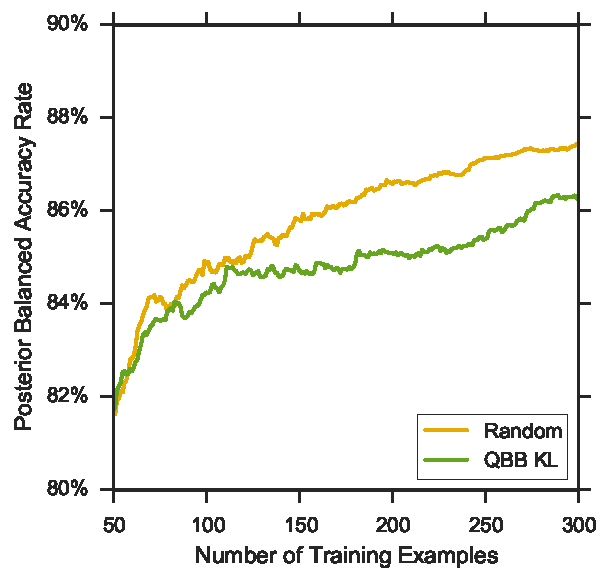
\includegraphics[width=0.99\textwidth]{figures/5_active/sdss_bl_ind_lower}
		\caption{Worse than random sampling}
		\label{fig:sdss_bl_ind_lower}
	\end{subfigure}%
	\begin{subfigure}{.5\textwidth}
		\centering
		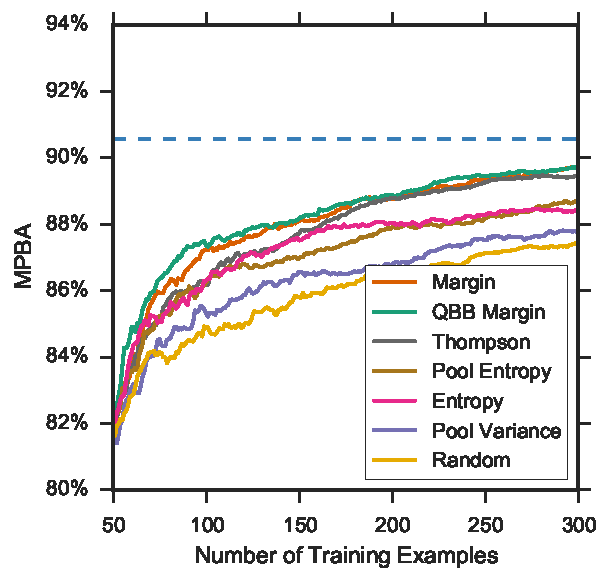
\includegraphics[width=0.99\linewidth]{figures/5_active/sdss_bl_ind_upper}
		\caption{Better than random sampling}
		\label{fig:sdss_bl_ind_upper}
	\end{subfigure}
	\caption[Learning curves with heuristics (SDSS, balanced, logistic)]{
		Learning curves with heuristics (SDSS dataset, balanced pool, logistic regression)}
	\label{fig:sdss_bl_ind}
\end{figure}

\begin{figure}[p]
	\centering
	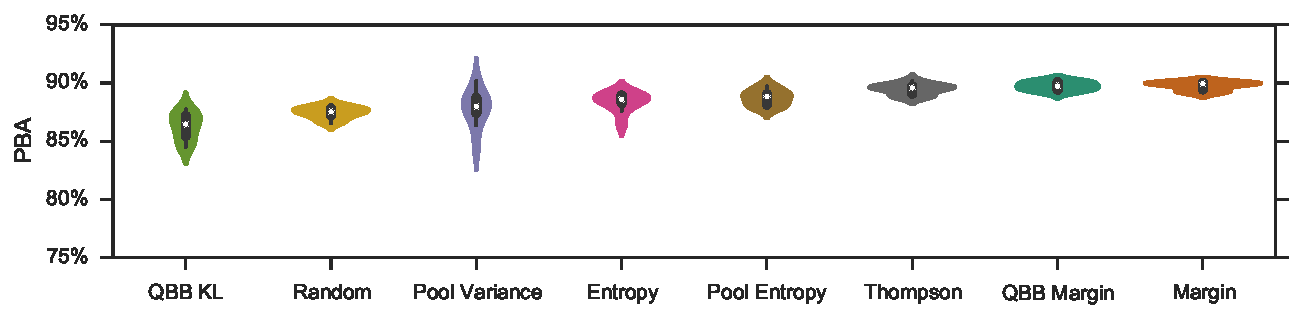
\includegraphics[width=\textwidth]{figures/5_active/sdss_bl_ind_violin}
	\caption[Violin plots of final accuracy rates (SDSS, balanced, logistic)]{
		Violin plots of final accuracy rates (SDSS dataset, balanced pool, logistic regression)}
	\label{fig:sdss_bl_ind_violin}
\end{figure}

\begin{figure}[p]
	\centering
	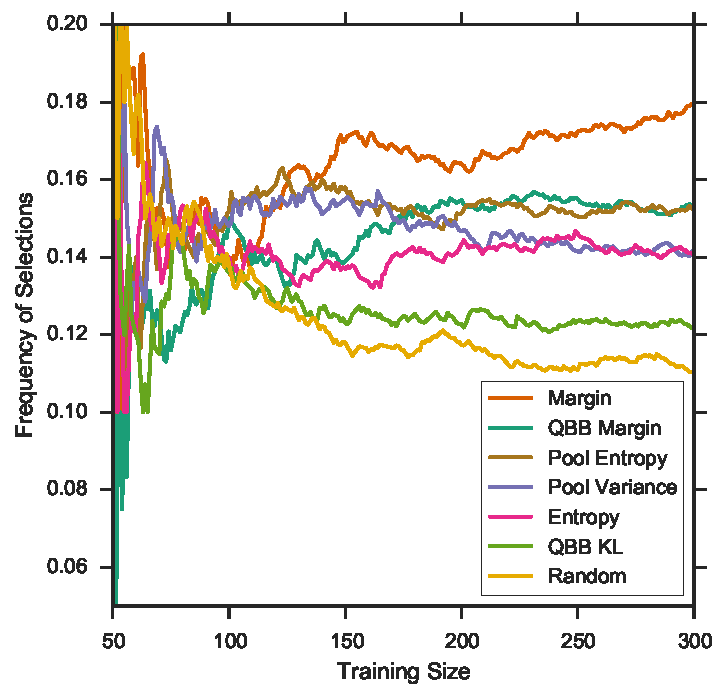
\includegraphics[width=\textwidth]{figures/5_thompson/sdss_bl_frequencies}
	\caption[Heuristic selection frequency (SDSS, balanced, logistic)]{
		Heuristic selection frequency (SDSS dataset, balanced pool, logistic regression)}
	\label{fig:sdss_bl_frequencies}
\end{figure}

\begin{figure}[p]
	\centering
	\begin{subfigure}{.5\textwidth}
		\centering
		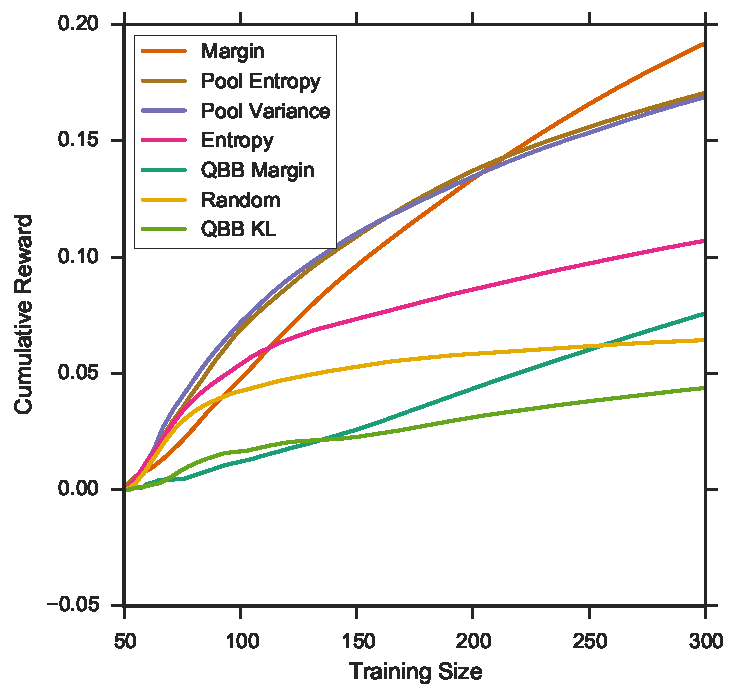
\includegraphics[width=0.99\textwidth]{figures/5_thompson/sdss_bl_sum_rewards}
		\caption{Cumulative reward}
		\label{fig:sdss_bl_sum_rewards}
	\end{subfigure}%
	\begin{subfigure}{.5\textwidth}
		\centering
		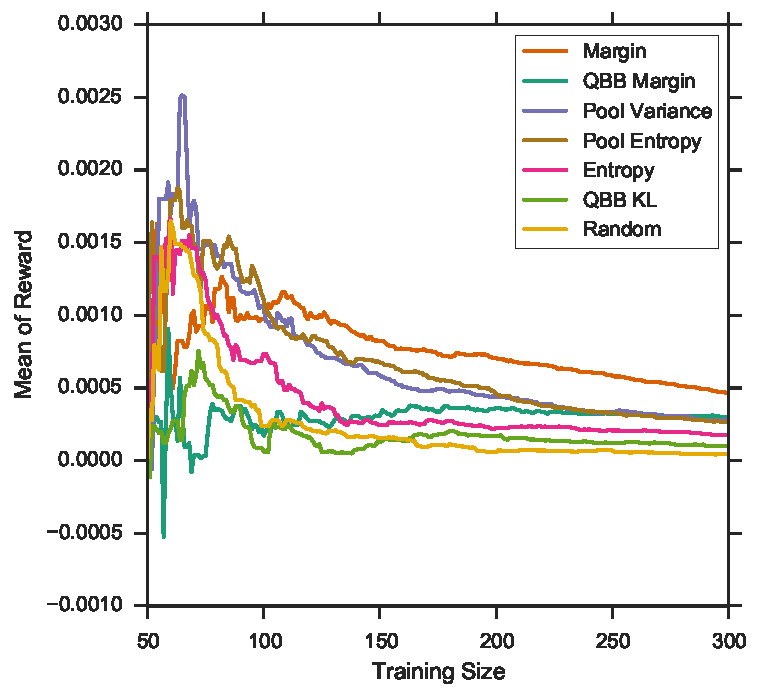
\includegraphics[width=0.99\linewidth]{figures/5_thompson/sdss_bl_avg_rewards}
		\caption{Mean of reward}
		\label{fig:sdss_bl_avg_rewards}
	\end{subfigure}
	\caption[Reward of heuristics (SDSS, balanced, logistic)]{
		Reward of heuristics (SDSS dataset, balanced pool, logistic regression)}
	\label{fig:sdss_bl_rewards}
\end{figure}

%--------------------------------------------------------------------------------------------------
\begin{figure}[p]
	\centering
	\begin{subfigure}{.5\textwidth}
		\centering
		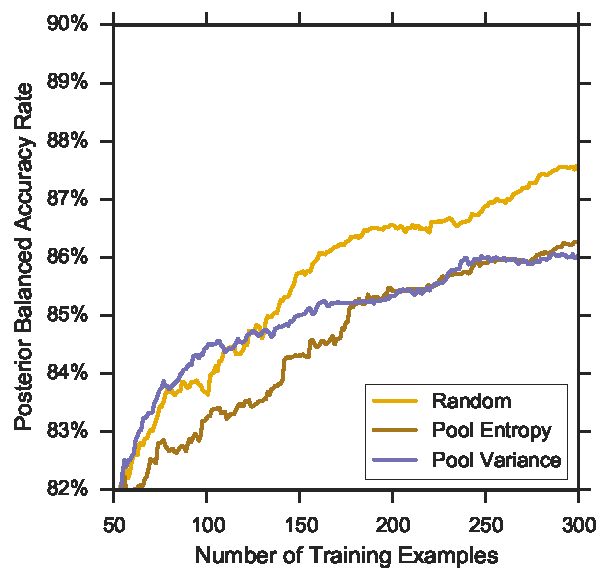
\includegraphics[width=0.99\textwidth]{figures/5_active/sdss_br_ind_lower}
		\caption{Worse than random sampling}
		\label{fig:sdss_br_ind_lower}
	\end{subfigure}%
	\begin{subfigure}{.5\textwidth}
		\centering
		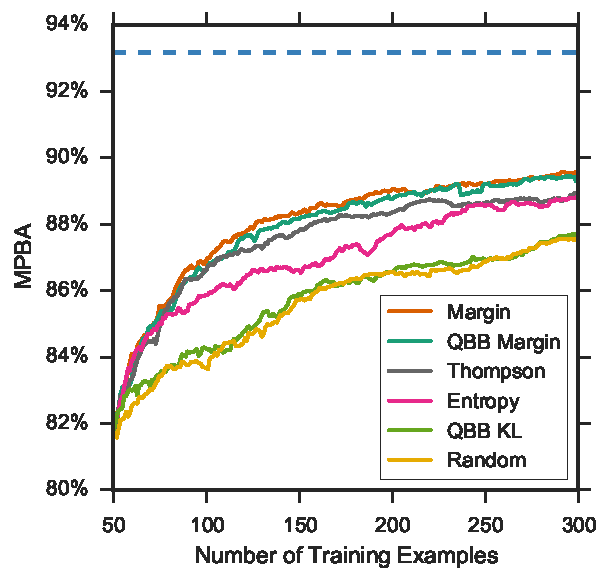
\includegraphics[width=0.99\linewidth]{figures/5_active/sdss_br_ind_upper}
		\caption{Better than random sampling}
		\label{fig:sdss_br_ind_upper}
	\end{subfigure}
	\caption[Learning curves with heuristics (SDSS, balanced, logistic)]{
		Learning curves with heuristics (SDSS dataset, balanced pool, logistic regression)}
	\label{fig:sdss_br_ind}
\end{figure}

\begin{figure}[p]
	\centering
	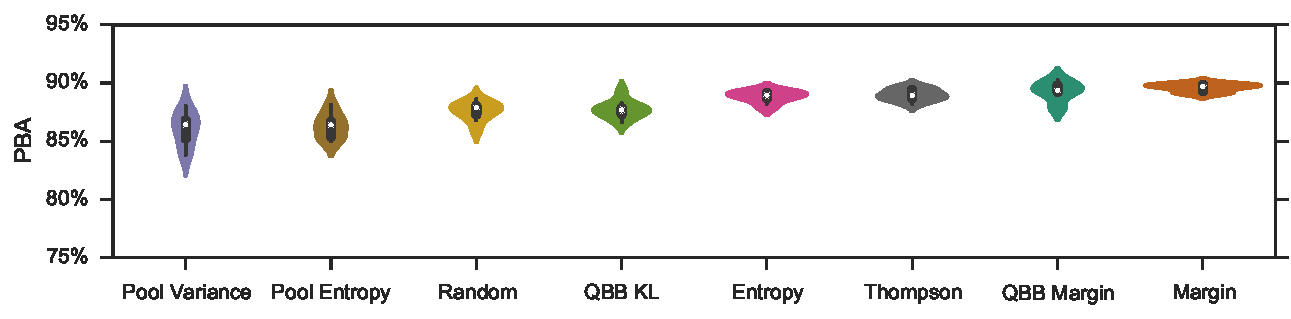
\includegraphics[width=\textwidth]{figures/5_active/sdss_br_ind_violin}
	\caption[Violin plots of final accuracy rates (SDSS, balanced, SVM RBF)]{
		Violin plots of final accuracy rates (SDSS dataset, balanced pool, SVM RBF)}
	\label{fig:sdss_br_ind_violin}
\end{figure}

\begin{figure}[p]
	\centering
	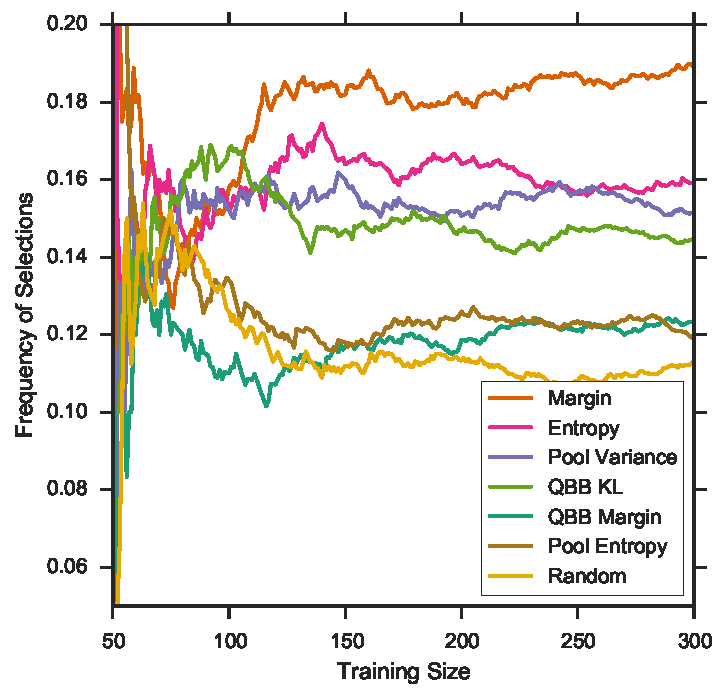
\includegraphics[width=\textwidth]{figures/5_thompson/sdss_br_frequencies}
	\caption[Heuristic selection frequency (SDSS, balanced, SVM RBF)]{
		Heuristic selection frequency (SDSS dataset, balanced pool, SVM RBF)}
	\label{fig:sdss_br_frequencies}
\end{figure}

\begin{figure}[p]
	\centering
	\begin{subfigure}{.5\textwidth}
		\centering
		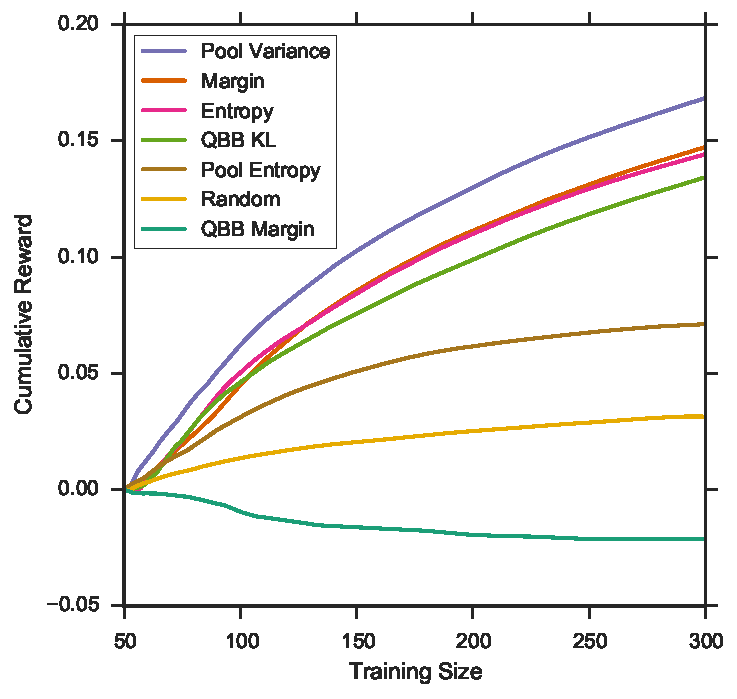
\includegraphics[width=0.99\textwidth]{figures/5_thompson/sdss_br_sum_rewards}
		\caption{Cumulative reward}
		\label{fig:sdss_br_sum_rewards}
	\end{subfigure}%
	\begin{subfigure}{.5\textwidth}
		\centering
		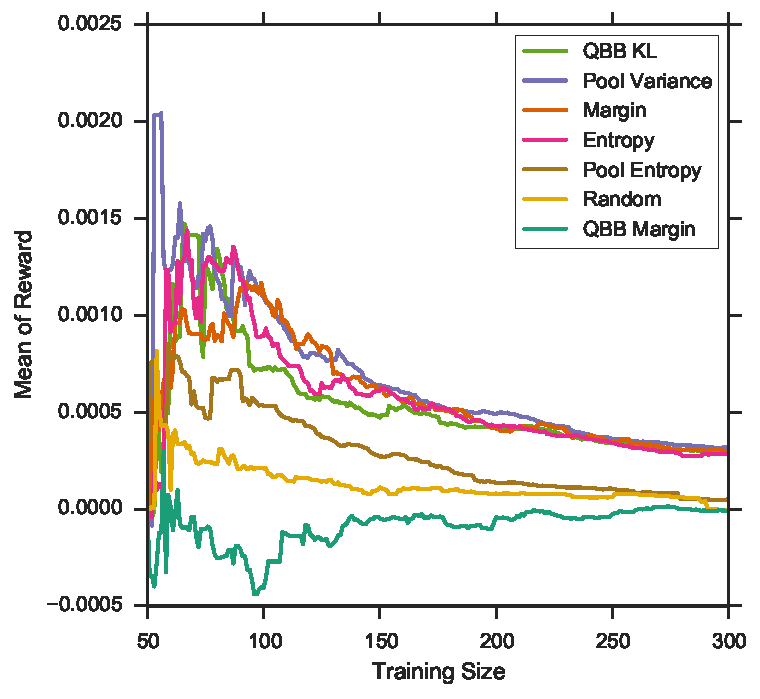
\includegraphics[width=0.99\linewidth]{figures/5_thompson/sdss_br_avg_rewards}
		\caption{Mean of reward}
		\label{fig:sdss_br_avg_rewards}
	\end{subfigure}
	\caption[Reward of heuristics (SDSS, balanced, SVM RBF)]{
		Reward of heuristics (SDSS dataset, balanced pool, SVM RBF)}
	\label{fig:sdss_br_rewards}
\end{figure}


%--------------------------------------------------------------------------------------------------
\begin{figure}[p]
	\centering
	\begin{subfigure}{.5\textwidth}
		\centering
		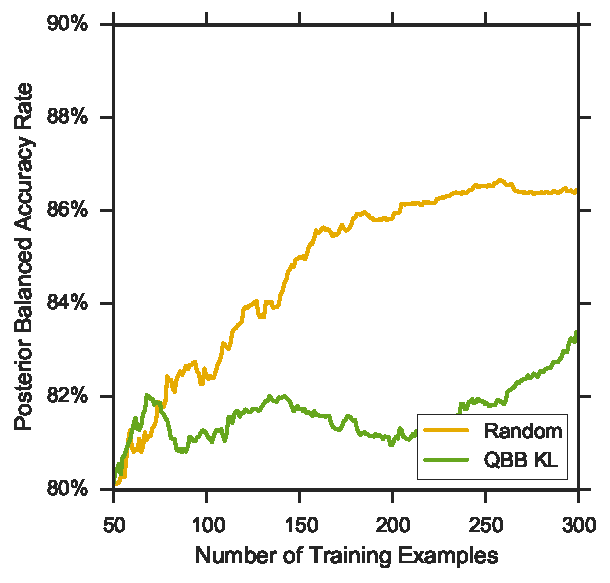
\includegraphics[width=0.99\textwidth]{figures/5_active/sdss_ul_ind_lower}
		\caption{Worse than random sampling}
		\label{fig:sdss_ul_ind_lower}
	\end{subfigure}%
	\begin{subfigure}{.5\textwidth}
		\centering
		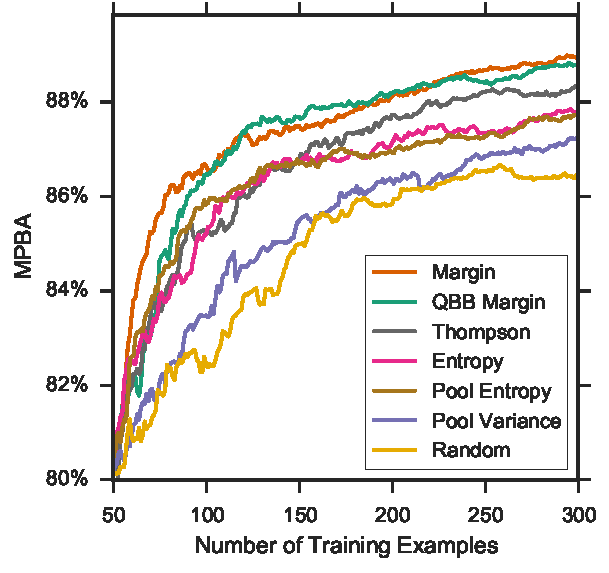
\includegraphics[width=0.99\linewidth]{figures/5_active/sdss_ul_ind_upper}
		\caption{Better than random sampling}
		\label{fig:sdss_ul_ind_upper}
	\end{subfigure}
	\caption[Learning curves with heuristics (SDSS, balanced, logistic)]{
		Learning curves with heuristics (SDSS dataset, unbalanced pool, logistic regression)}
	\label{fig:sdss_ul_ind}
\end{figure}

\begin{figure}[p]
	\centering
	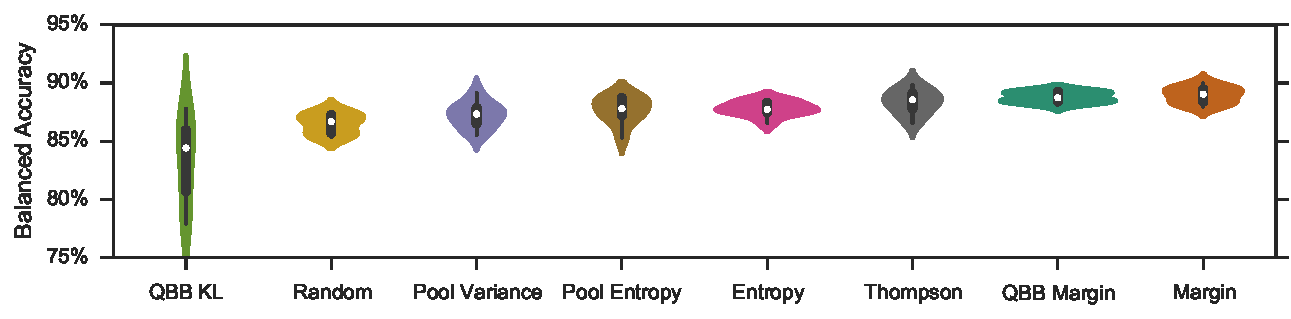
\includegraphics[width=\textwidth]{figures/5_active/sdss_ul_ind_violin}
	\caption[Violin plots of final accuracy rates (SDSS, unbalanced, logistic)]{
		Violin plots of final accuracy rates (SDSS dataset, unbalanced pool, logistic regression)}
	\label{fig:sdss_ul_ind_violin}
\end{figure}

\begin{figure}[p]
	\centering
	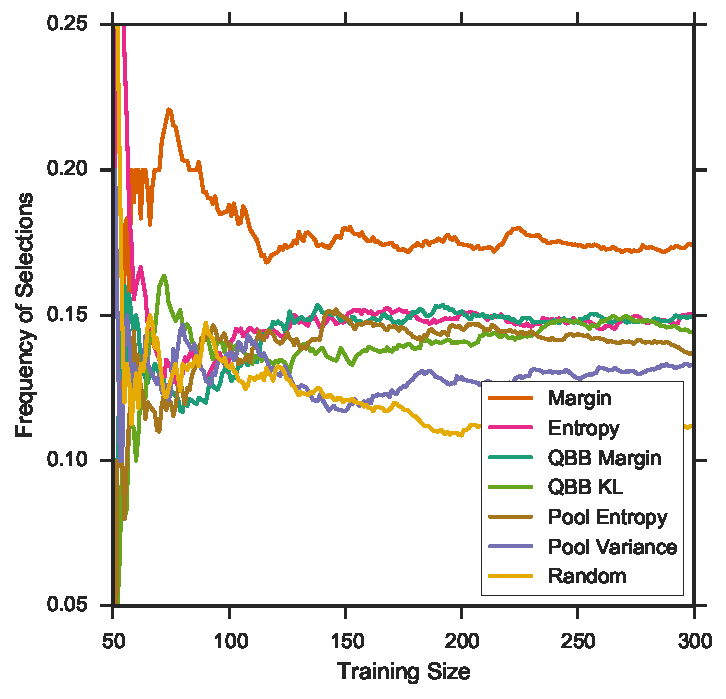
\includegraphics[width=\textwidth]{figures/5_thompson/sdss_ul_frequencies}
	\caption[Heuristic selection frequency (SDSS, unbalanced, logistic)]{
		Heuristic selection frequency (SDSS dataset, unbalanced pool, logistic regression)}
	\label{fig:sdss_ul_frequencies}
\end{figure}

\begin{figure}[p]
	\centering
	\begin{subfigure}{.5\textwidth}
		\centering
		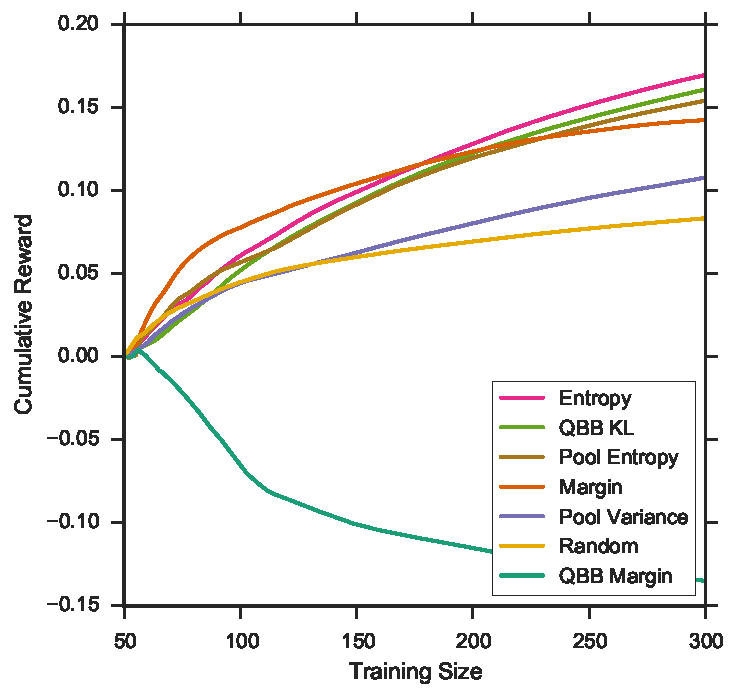
\includegraphics[width=0.99\textwidth]{figures/5_thompson/sdss_ul_sum_rewards}
		\caption{Cumulative reward}
		\label{fig:sdss_ul_sum_rewards}
	\end{subfigure}%
	\begin{subfigure}{.5\textwidth}
		\centering
		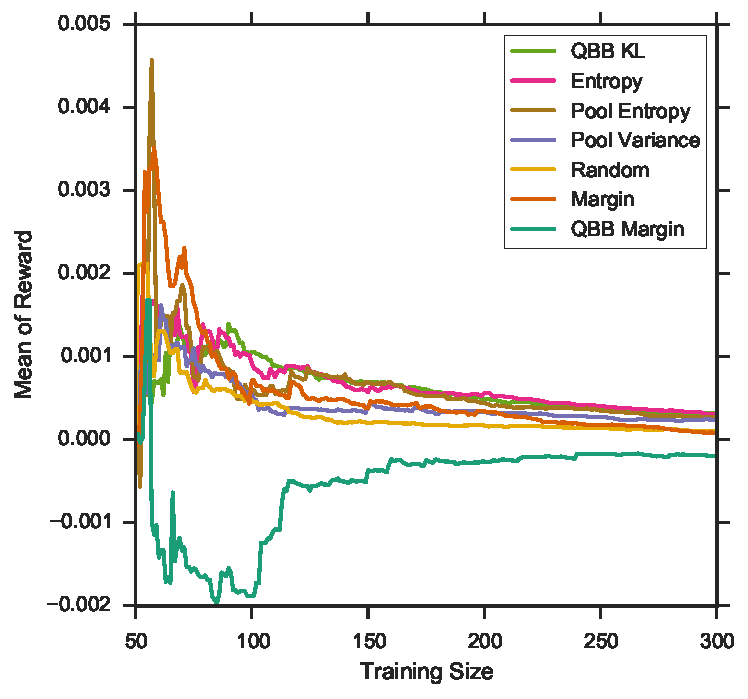
\includegraphics[width=0.99\linewidth]{figures/5_thompson/sdss_ul_avg_rewards}
		\caption{Mean of reward}
		\label{fig:sdss_ul_avg_rewards}
	\end{subfigure}
	\caption[Reward of heuristics (SDSS, unbalanced, logistic)]{
		Reward of heuristics (SDSS dataset, unbalanced pool, logistic regression)}
	\label{fig:sdss_ul_rewards}
\end{figure}

%--------------------------------------------------------------------------------------------------
\begin{figure}[p]
	\centering
	\begin{subfigure}{.5\textwidth}
		\centering
		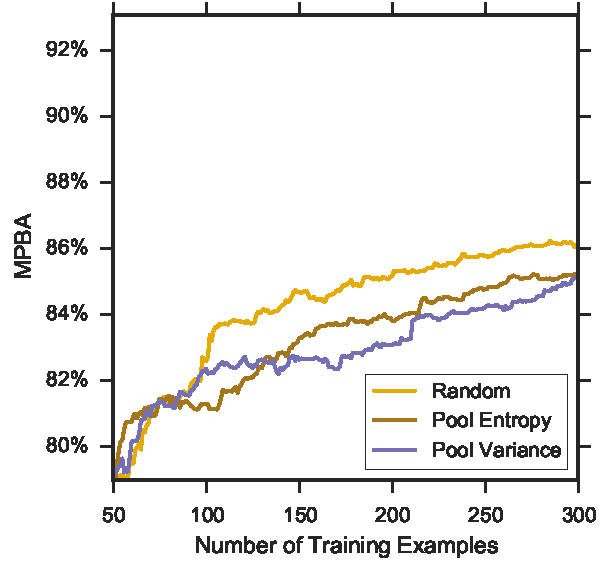
\includegraphics[width=0.99\textwidth]{figures/5_active/sdss_ur_ind_lower}
		\caption{Worse than random sampling}
		\label{fig:sdss_ur_ind_lower}
	\end{subfigure}%
	\begin{subfigure}{.5\textwidth}
		\centering
		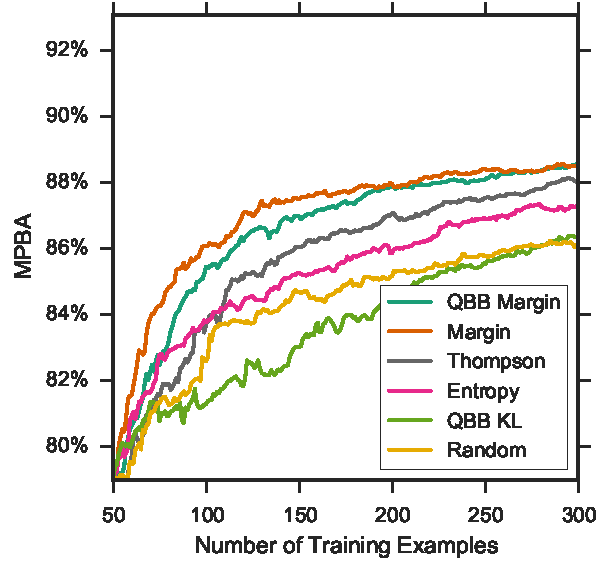
\includegraphics[width=0.99\linewidth]{figures/5_active/sdss_ur_ind_upper}
		\caption{Better than random sampling}
		\label{fig:sdss_ur_ind_upper}
	\end{subfigure}
	\caption[Learning curves with heuristics (SDSS, unbalanced, logistic)]{
		Learning curves with heuristics (SDSS dataset, unbalanced pool, logistic regression)}
	\label{fig:sdss_ur_ind}
\end{figure}

\begin{figure}[p]
	\centering
	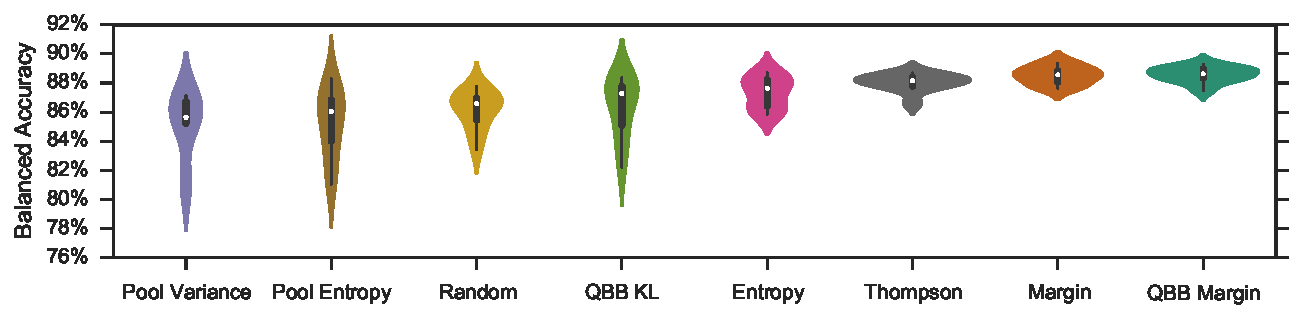
\includegraphics[width=\textwidth]{figures/5_active/sdss_ur_ind_violin}
	\caption[Violin plots of final accuracy rates (SDSS, unbalanced, SVM RBF)]{
		Violin plots of final accuracy rates (SDSS dataset, unbalanced pool, SVM RBF)}
	\label{fig:sdss_ur_ind_violin}
\end{figure}

\begin{figure}[p]
	\centering
	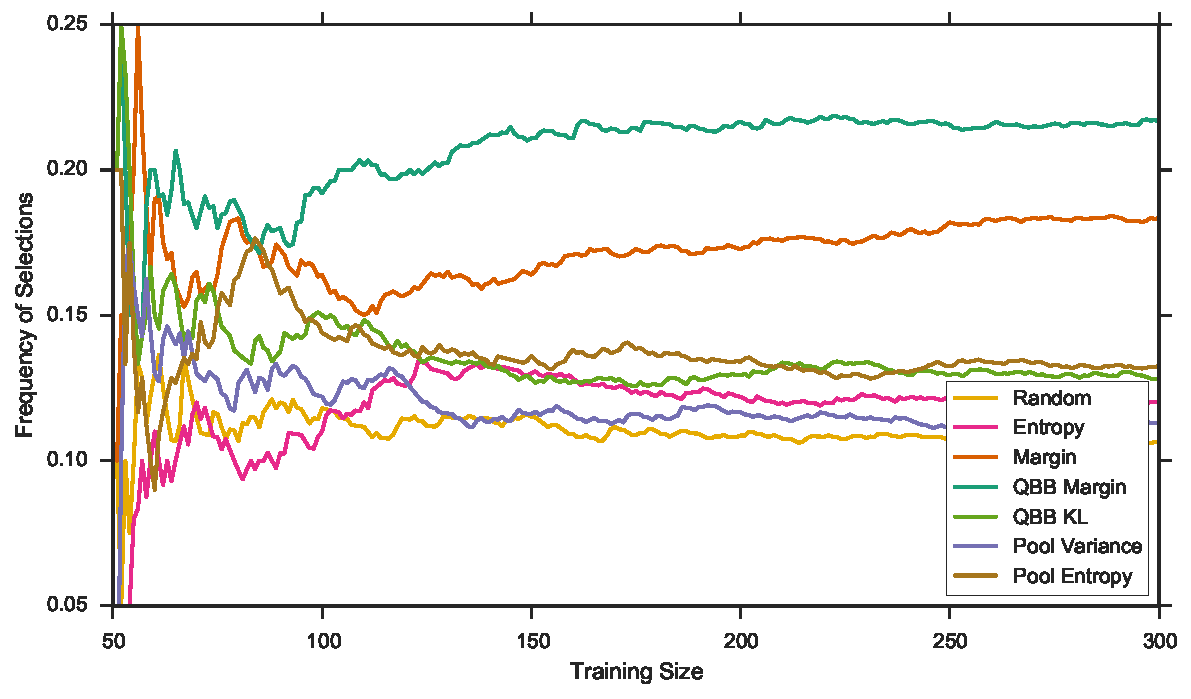
\includegraphics[width=\textwidth]{figures/5_thompson/sdss_ur_frequencies}
	\caption[Heuristic selection frequency (SDSS, unbalanced, SVM RBF)]{
		Heuristic selection frequency (SDSS dataset, unbalanced pool, SVM RBF)}
	\label{fig:sdss_ur_frequencies}
\end{figure}

\begin{figure}[p]
	\centering
	\begin{subfigure}{.5\textwidth}
		\centering
		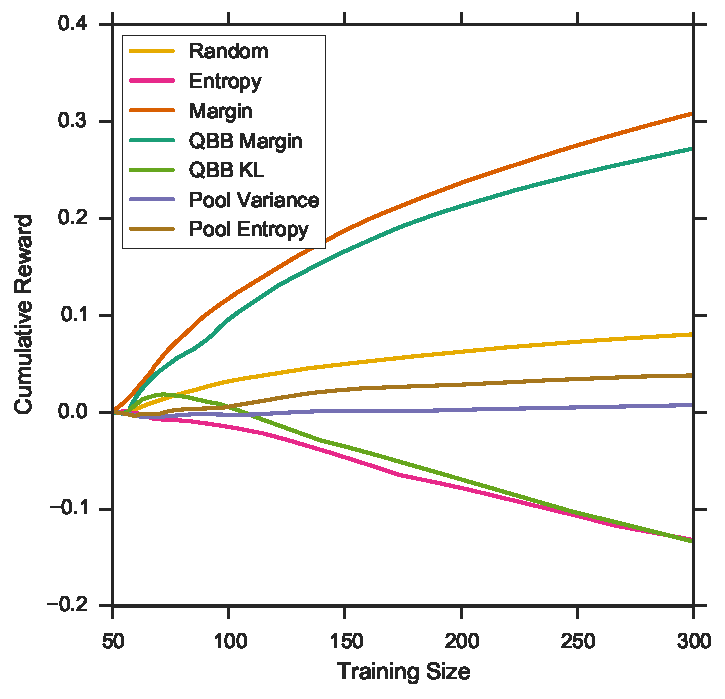
\includegraphics[width=0.99\textwidth]{figures/5_thompson/sdss_ur_sum_rewards}
		\caption{Cumulative reward}
		\label{fig:sdss_ur_sum_rewards}
	\end{subfigure}%
	\begin{subfigure}{.5\textwidth}
		\centering
		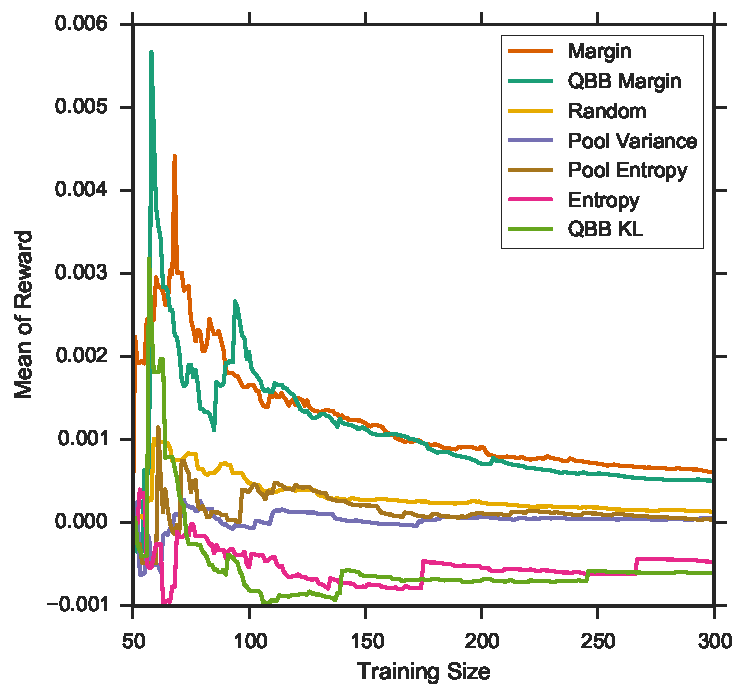
\includegraphics[width=0.99\linewidth]{figures/5_thompson/sdss_ur_avg_rewards}
		\caption{Mean of reward}
		\label{fig:sdss_ur_avg_rewards}
	\end{subfigure}
	\caption[Reward of heuristics (SDSS, unbalanced, SVM RBF)]{
		Reward of heuristics (SDSS dataset, unbalanced pool, SVM RBF)}
	\label{fig:sdss_ur_rewards}
\end{figure}



\clearpage
% % % % % % % % % % % % % % % % % % % % % % % % % % % % % % % % % % % % % % % % % % % % % % % % % %
\subsection{Learning with the VST ATLAS Dataset}

%--------------------------------------------------------------------------------------------------
\begin{figure}[p]
	\centering
	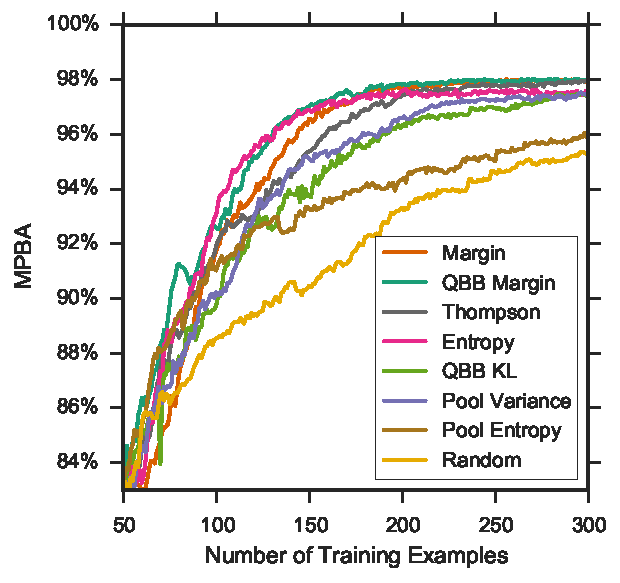
\includegraphics[width=0.5\textwidth]{figures/5_active/vstatlas_bl_ind_upper}
	\caption[Learning curves with heuristics (VST ATLAS, balanced, logistic)]{
		Learning curves with heuristics (VST ATLAS dataset, balanced pool, logistic regression)}
	\label{fig:vstatlas_bl_ind_upper}
\end{figure}

%\begin{figure}[p]
%	\centering
%	\begin{subfigure}{.5\textwidth}
%		\centering
%		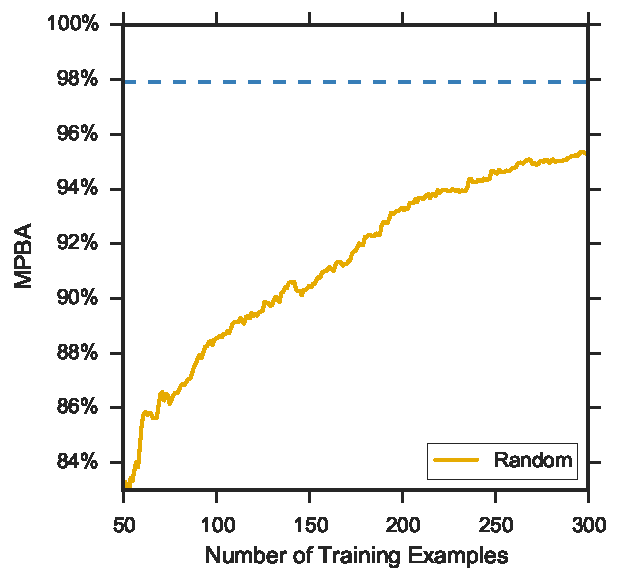
\includegraphics[width=0.99\textwidth]{figures/5_active/vstatlas_bl_ind_lower}
%		\caption{Worse than random sampling}
%		\label{fig:vstatlas_bl_ind_lower}
%	\end{subfigure}%
%	\begin{subfigure}{.5\textwidth}
%		\centering
%		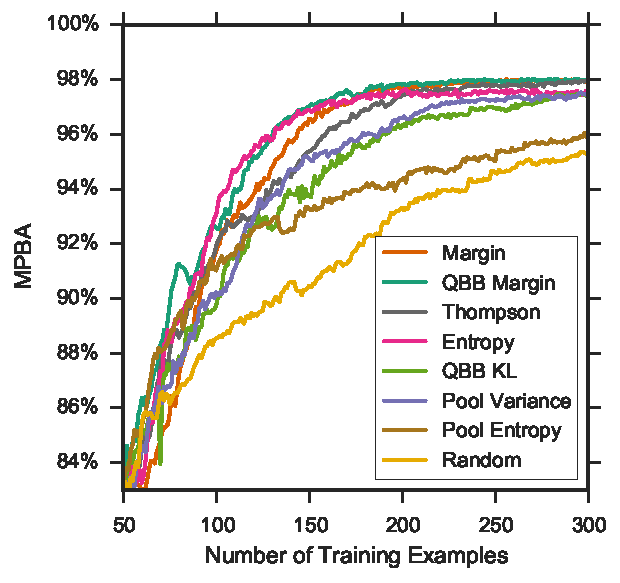
\includegraphics[width=0.99\linewidth]{figures/5_active/vstatlas_bl_ind_upper}
%		\caption{Better than random sampling}
%		\label{fig:vstatlas_bl_ind_upper}
%	\end{subfigure}
%	\caption[Learning curves with heuristics (VST ATLAS, balanced, logistic)]{
%		Learning curves with heuristics (VST ATLAS, balanced pool, logistic regression)}
%	\label{fig:vstatlas_bl_ind}
%\end{figure}

\begin{figure}[p]
	\centering
	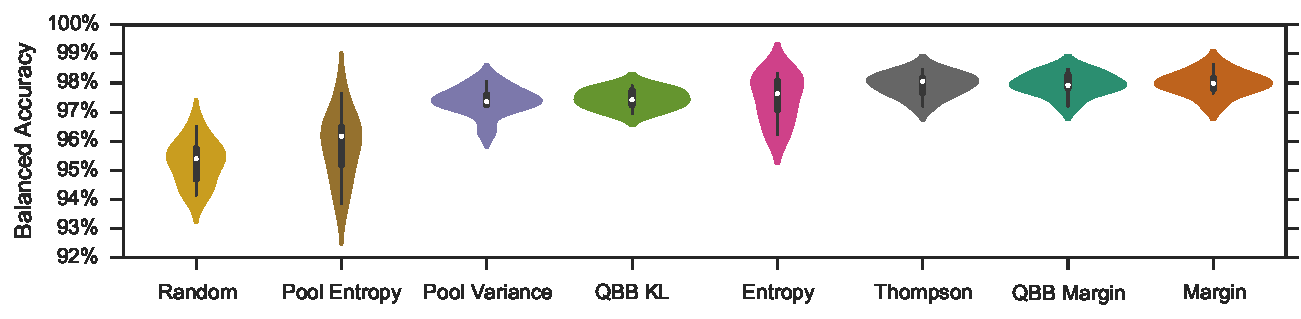
\includegraphics[width=\textwidth]{figures/5_active/vstatlas_bl_ind_violin}
	\caption[Violin plots of final accuracy rates (VST ATLAS, balanced, logistic)]{
		Violin plots of final accuracy rates (VST ATLAS dataset, balanced pool, logistic regression)}
	\label{fig:vstatlas_bl_ind_violin}
\end{figure}

\begin{figure}[p]
	\centering
	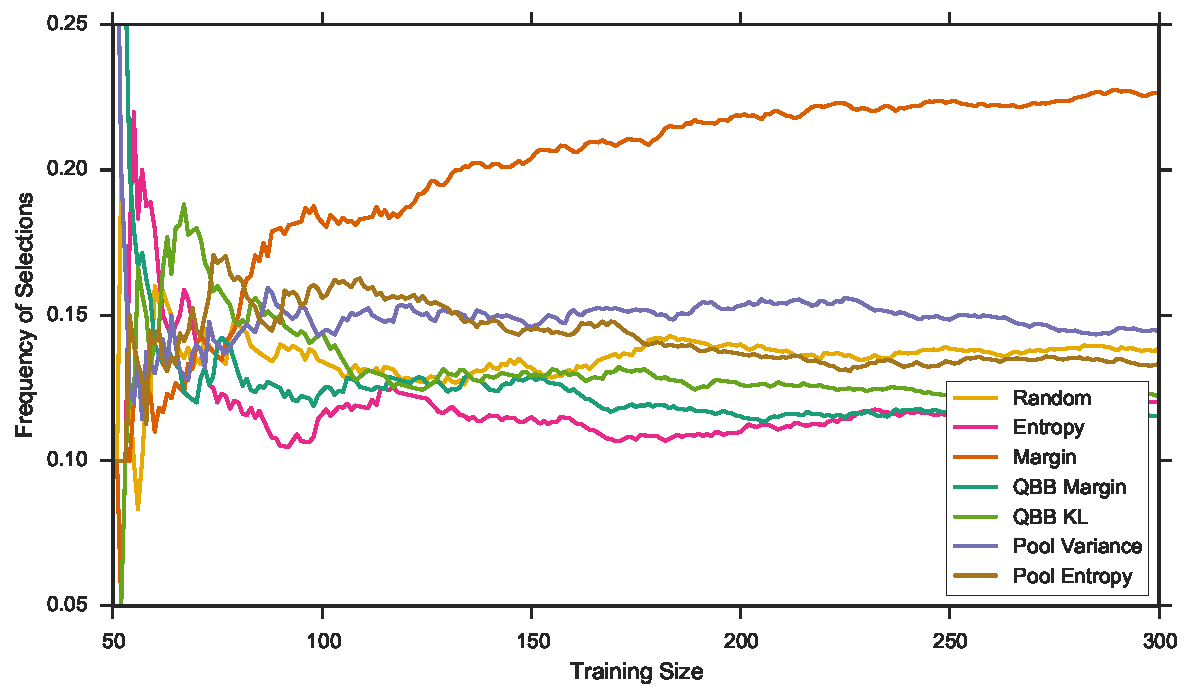
\includegraphics[width=\textwidth]{figures/5_thompson/vstatlas_bl_frequencies}
	\caption[Heuristic selection frequency (VST ATLAS, balanced, logistic)]{
		Heuristic selection frequency (VST ATLAS dataset, balanced pool, logistic regression)}
	\label{fig:vstatlas_bl_frequencies}
\end{figure}

\begin{figure}[p]
	\centering
	\begin{subfigure}{.5\textwidth}
		\centering
		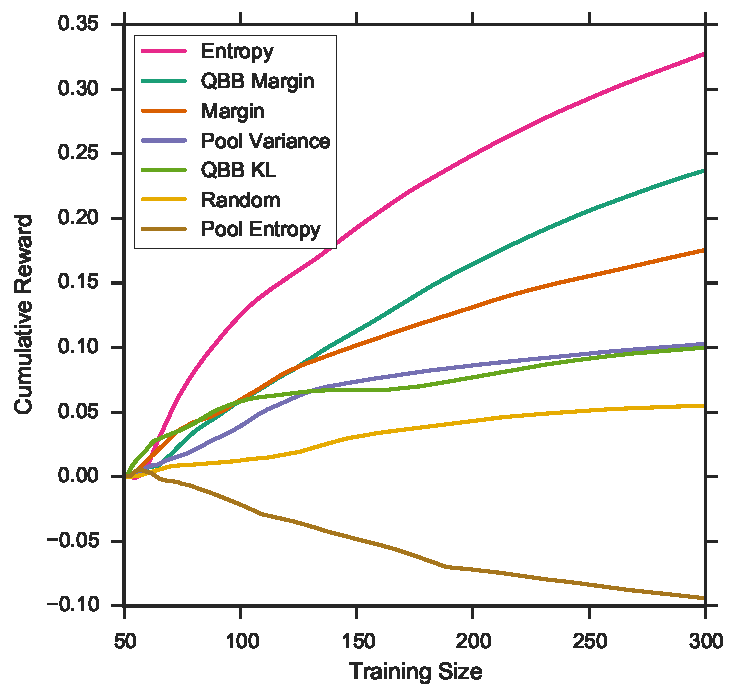
\includegraphics[width=0.99\textwidth]{figures/5_thompson/vstatlas_bl_sum_rewards}
		\caption{Cumulative reward}
		\label{fig:vstatlas_bl_sum_rewards}
	\end{subfigure}%
	\begin{subfigure}{.5\textwidth}
		\centering
		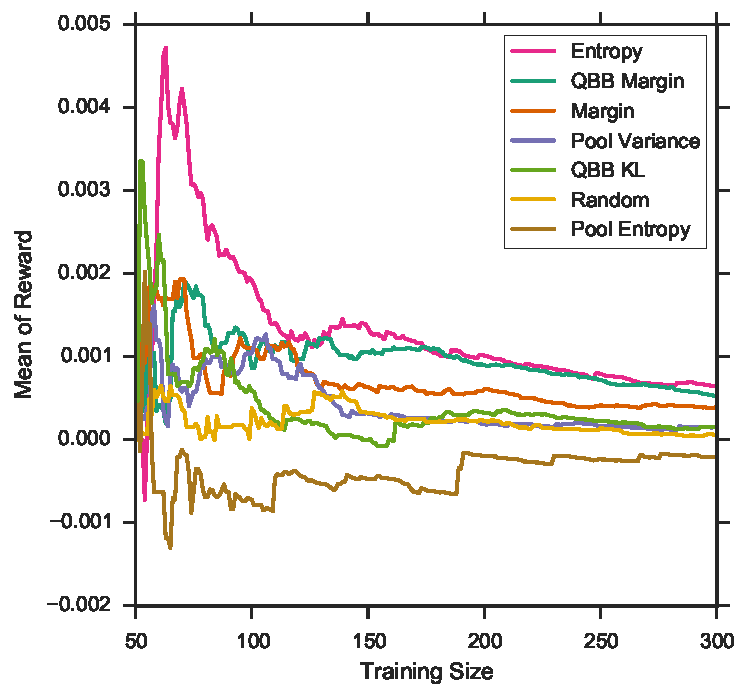
\includegraphics[width=0.99\linewidth]{figures/5_thompson/vstatlas_bl_avg_rewards}
		\caption{Mean of reward}
		\label{fig:vstatlas_bl_avg_rewards}
	\end{subfigure}
	\caption[Reward of heuristics (VST ATLAS, balanced, logistic)]{
		Reward of heuristics (VST ATLAS dataset, balanced pool, logistic regression)}
	\label{fig:vstatlas_bl_rewards}
\end{figure}

%--------------------------------------------------------------------------------------------------
\begin{figure}[p]
	\centering
	\begin{subfigure}{.5\textwidth}
		\centering
		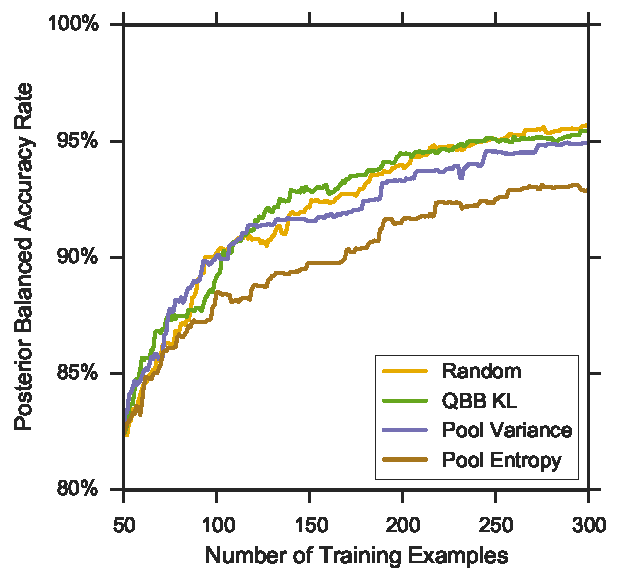
\includegraphics[width=0.99\textwidth]{figures/5_active/vstatlas_br_ind_lower}
		\caption{Worse than random sampling}
		\label{fig:vstatlas_br_ind_lower}
	\end{subfigure}%
	\begin{subfigure}{.5\textwidth}
		\centering
		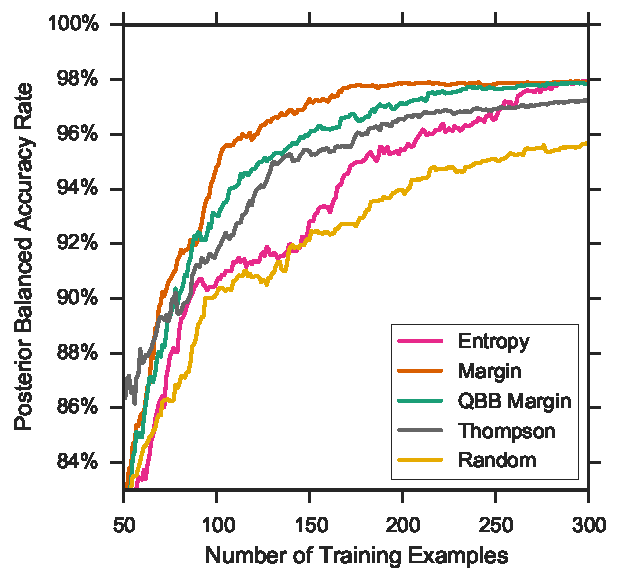
\includegraphics[width=0.99\linewidth]{figures/5_active/vstatlas_br_ind_upper}
		\caption{Better than random sampling}
		\label{fig:vstatlas_br_ind_upper}
	\end{subfigure}
	\caption[Learning curves with heuristics (VST ATLAS, balanced, logistic)]{
		Learning curves with heuristics (VST ATLAS dataset, balanced pool, logistic regression)}
	\label{fig:vstatlas_br_ind}
\end{figure}

\begin{figure}[p]
	\centering
	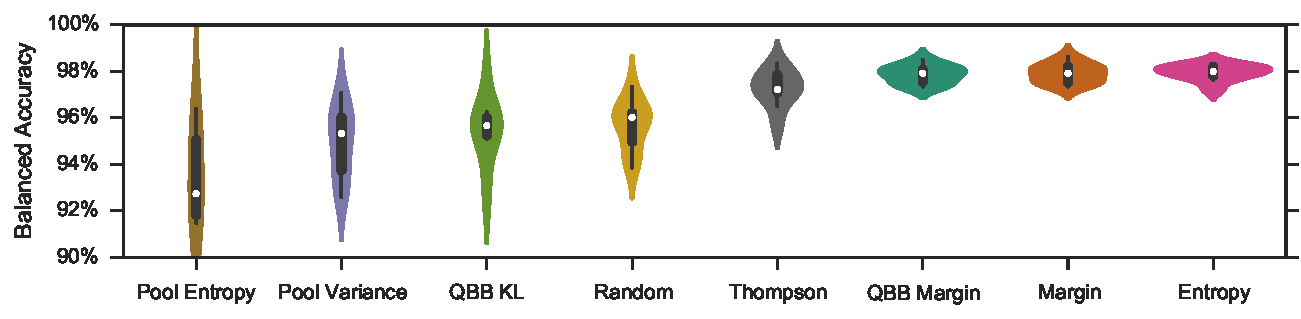
\includegraphics[width=\textwidth]{figures/5_active/vstatlas_br_ind_violin}
	\caption[Violin plots of final accuracy rates (VST ATLAS, balanced, SVM RBF)]{
		Violin plots of final accuracy rates (VST ATLAS dataset, balanced pool, SVM RBF)}
	\label{fig:vstatlas_br_ind_violin}
\end{figure}

\begin{figure}[p]
	\centering
	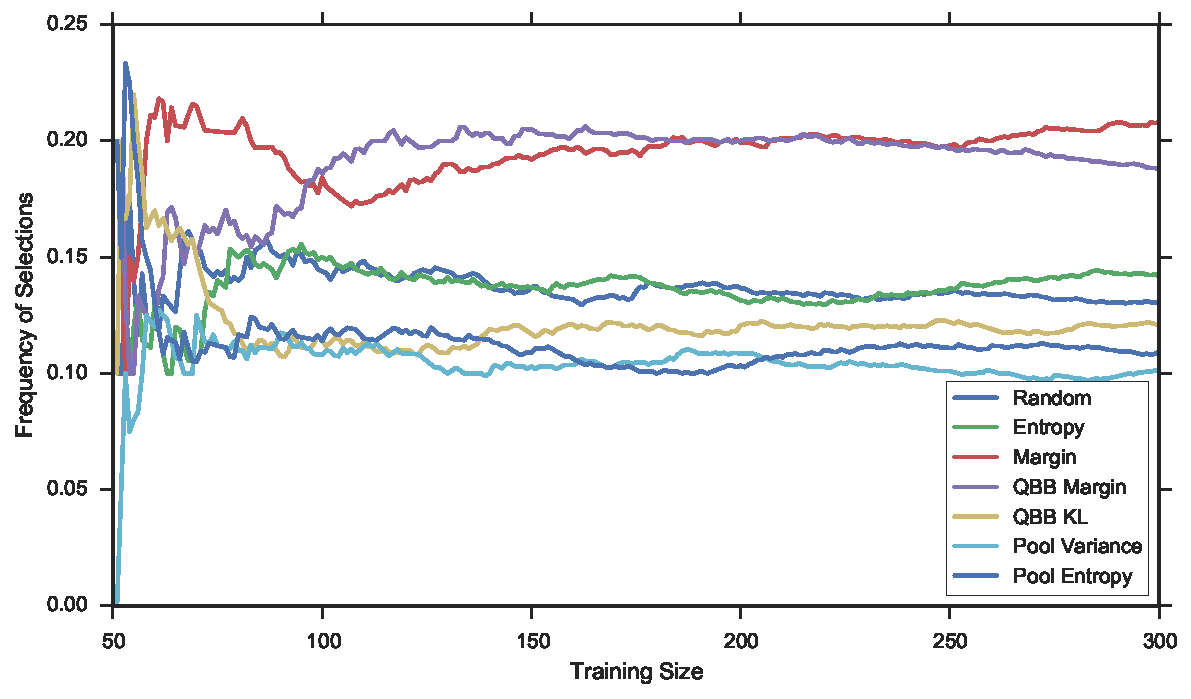
\includegraphics[width=\textwidth]{figures/5_thompson/vstatlas_br_frequencies}
	\caption[Heuristic selection frequency (VST ATLAS, balanced, SVM RBF)]{
		Heuristic selection frequency (VST ATLAS dataset, balanced pool, SVM RBF)}
	\label{fig:vstatlas_br_frequencies}
\end{figure}

\begin{figure}[p]
	\centering
	\begin{subfigure}{.5\textwidth}
		\centering
		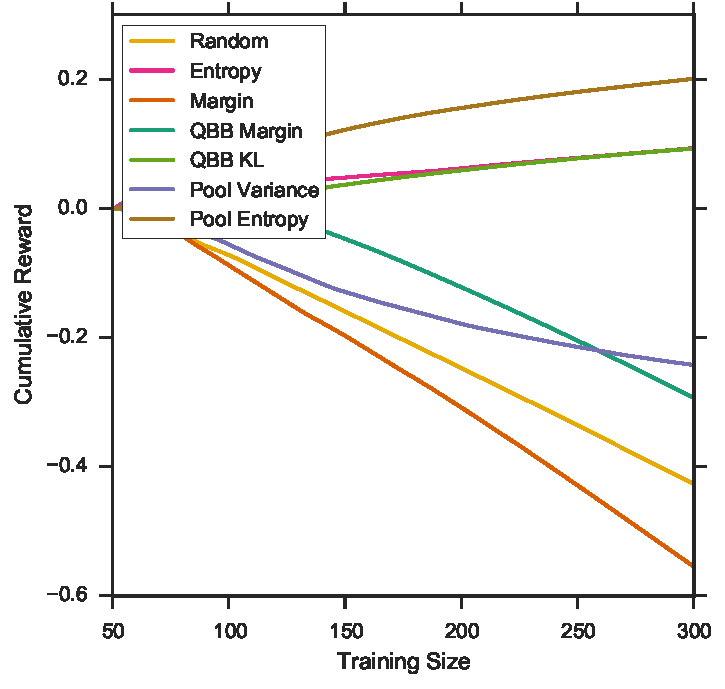
\includegraphics[width=0.99\textwidth]{figures/5_thompson/vstatlas_br_sum_rewards}
		\caption{Cumulative reward}
		\label{fig:vstatlas_br_sum_rewards}
	\end{subfigure}%
	\begin{subfigure}{.5\textwidth}
		\centering
		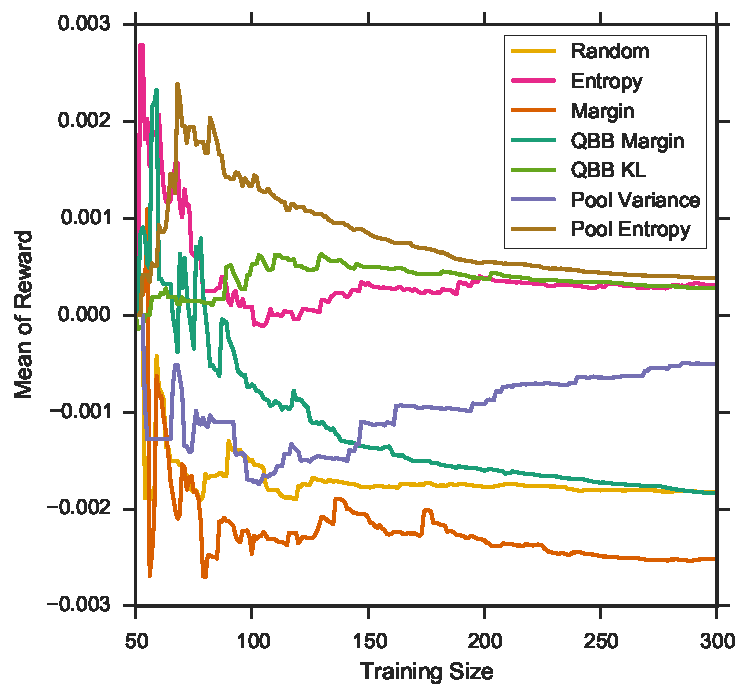
\includegraphics[width=0.99\linewidth]{figures/5_thompson/vstatlas_br_avg_rewards}
		\caption{Mean of reward}
		\label{fig:vstatlas_br_avg_rewards}
	\end{subfigure}
	\caption[Reward of heuristics (VST ATLAS, balanced, SVM RBF)]{
		Reward of heuristics (VST ATLAS dataset, balanced pool, SVM RBF)}
	\label{fig:vstatlas_br_rewards}
\end{figure}


%--------------------------------------------------------------------------------------------------
\begin{figure}[p]
	\centering
	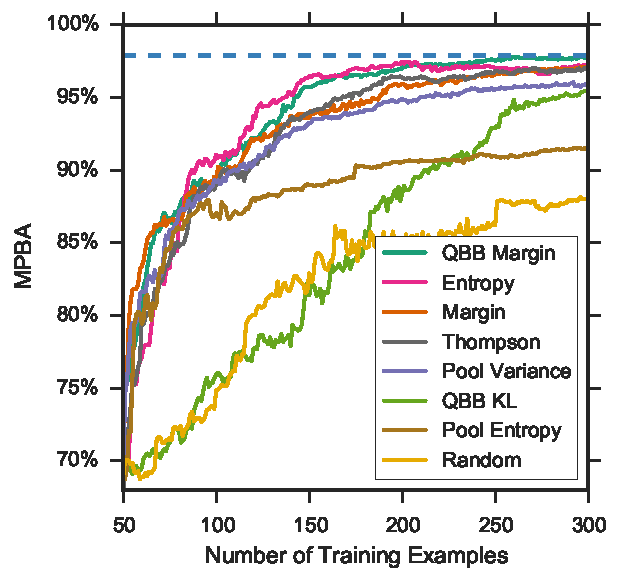
\includegraphics[width=0.5\textwidth]{figures/5_active/vstatlas_ul_ind_upper}
	\caption[Learning curves with heuristics (VST ATLAS, unbalanced, logistic)]{
		Learning curves with heuristics (VST ATLAS dataset, unbalanced pool, logistic regression)}
	\label{fig:vstatlas_ul_ind_upper}
\end{figure}


%\begin{figure}[p]
%	\centering
%	\begin{subfigure}{.5\textwidth}
%		\centering
%		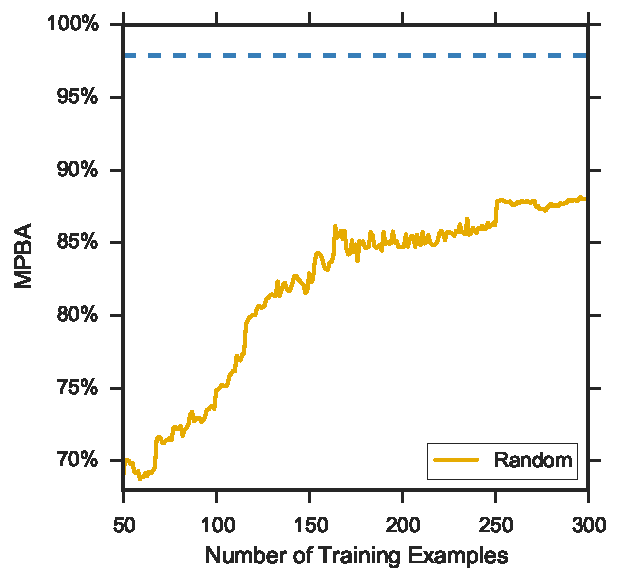
\includegraphics[width=0.99\textwidth]{figures/5_active/vstatlas_ul_ind_lower}
%		\caption{Worse than random sampling}
%		\label{fig:vstatlas_ul_ind_lower}
%	\end{subfigure}%
%	\begin{subfigure}{.5\textwidth}
%		\centering
%		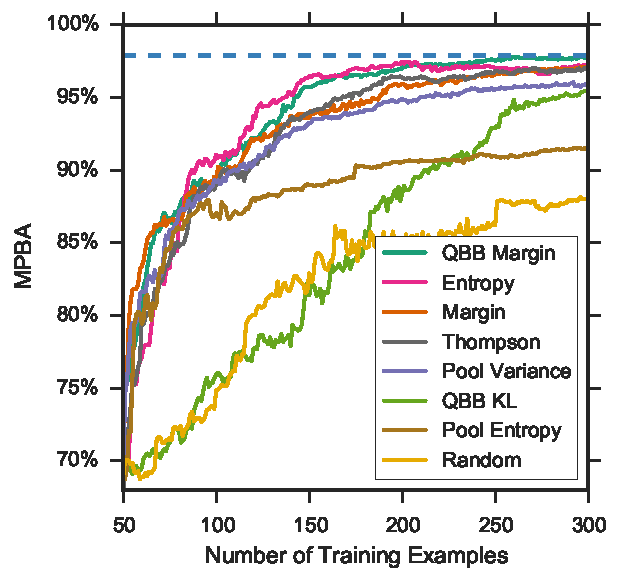
\includegraphics[width=0.99\linewidth]{figures/5_active/vstatlas_ul_ind_upper}
%		\caption{Better than random sampling}
%		\label{fig:vstatlas_ul_ind_upper}
%	\end{subfigure}
%	\caption[Learning curves with heuristics (VST ATLAS, unbalanced, logistic)]{
%		Learning curves with heuristics (VST ATLAS, unbalanced pool, logistic regression)}
%	\label{fig:vstatlas_ul_ind}
%\end{figure}

\begin{figure}[p]
	\centering
	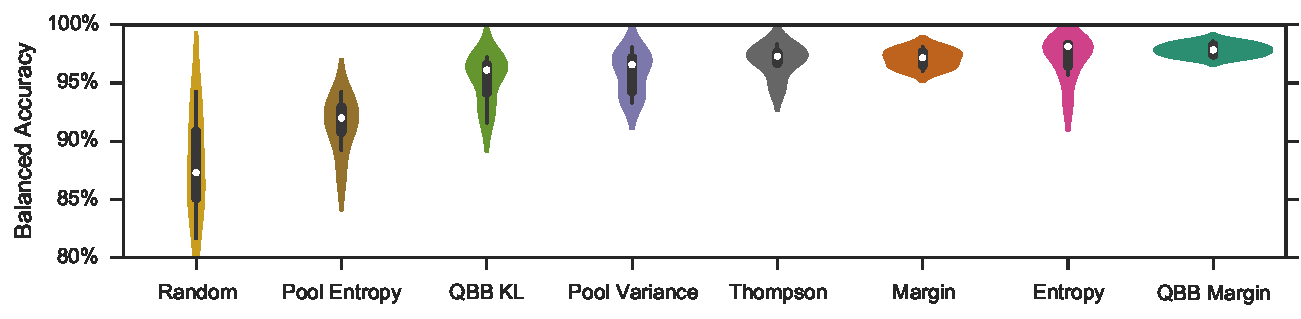
\includegraphics[width=\textwidth]{figures/5_active/vstatlas_ul_ind_violin}
	\caption[Violin plots of final accuracy rates (VST ATLAS, unbalanced, logistic)]{
		Violin plots of final accuracy rates (VST ATLAS dataset, unbalanced pool, logistic regression)}
	\label{fig:vstatlas_ul_ind_violin}
\end{figure}

\begin{figure}[p]
	\centering
	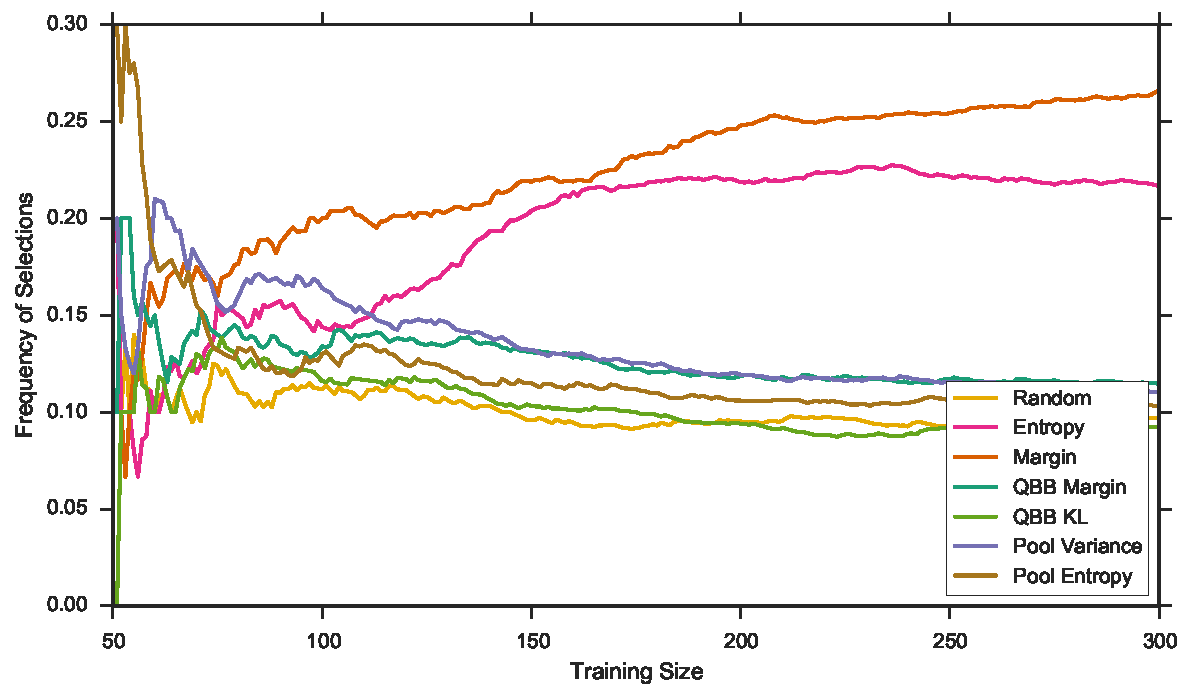
\includegraphics[width=\textwidth]{figures/5_thompson/vstatlas_ul_frequencies}
	\caption[Heuristic selection frequency (VST ATLAS, unbalanced, logistic)]{
		Heuristic selection frequency (VST ATLAS dataset, unbalanced pool, logistic regression)}
	\label{fig:vstatlas_ul_frequencies}
\end{figure}

\begin{figure}[p]
	\centering
	\begin{subfigure}{.5\textwidth}
		\centering
		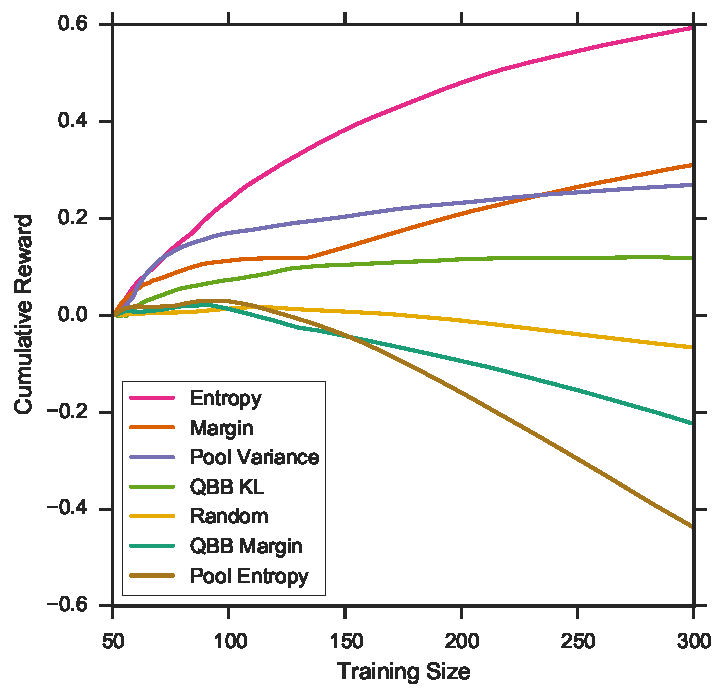
\includegraphics[width=0.99\textwidth]{figures/5_thompson/vstatlas_ul_sum_rewards}
		\caption{Cumulative reward}
		\label{fig:vstatlas_ul_sum_rewards}
	\end{subfigure}%
	\begin{subfigure}{.5\textwidth}
		\centering
		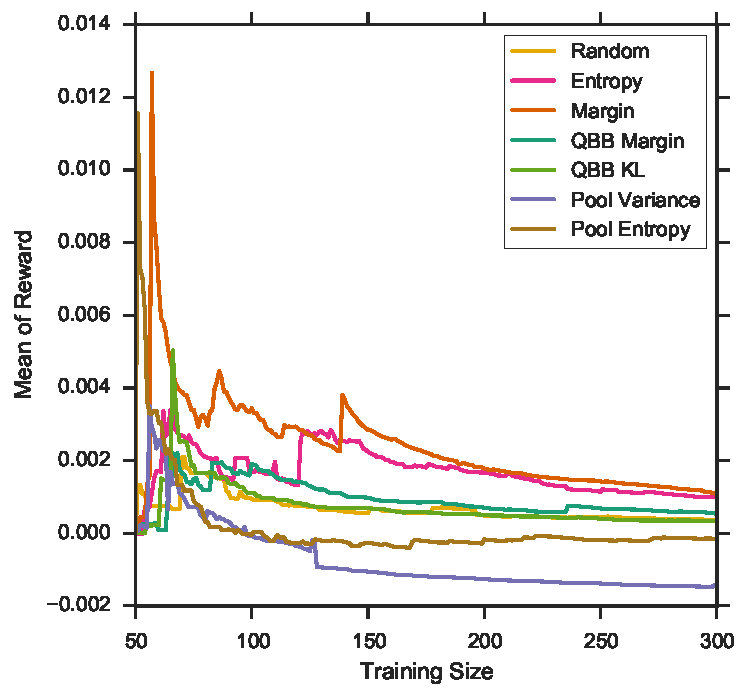
\includegraphics[width=0.99\linewidth]{figures/5_thompson/vstatlas_ul_avg_rewards}
		\caption{Mean of reward}
		\label{fig:vstatlas_ul_avg_rewards}
	\end{subfigure}
	\caption[Reward of heuristics (VST ATLAS, unbalanced, logistic)]{
		Reward of heuristics (VST ATLAS dataset, unbalanced pool, logistic regression)}
	\label{fig:vstatlas_ul_rewards}
\end{figure}

%--------------------------------------------------------------------------------------------------
\begin{figure}[p]
	\centering
	\begin{subfigure}{.5\textwidth}
		\centering
		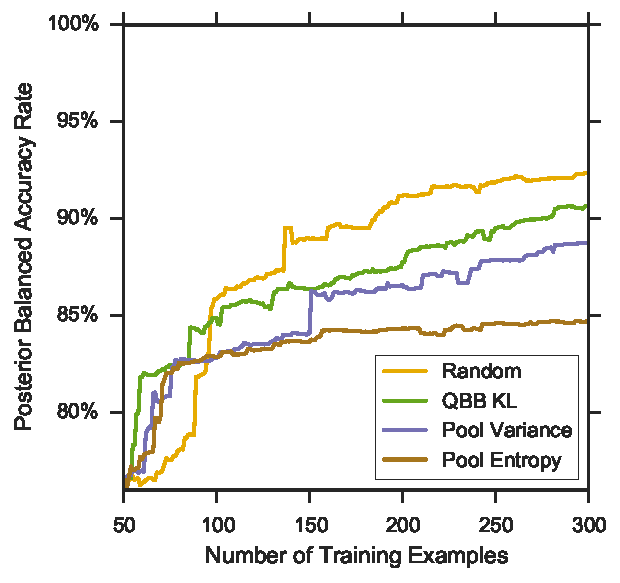
\includegraphics[width=0.99\textwidth]{figures/5_active/vstatlas_ur_ind_lower}
		\caption{Worse than random sampling}
		\label{fig:vstatlas_ur_ind_lower}
	\end{subfigure}%
	\begin{subfigure}{.5\textwidth}
		\centering
		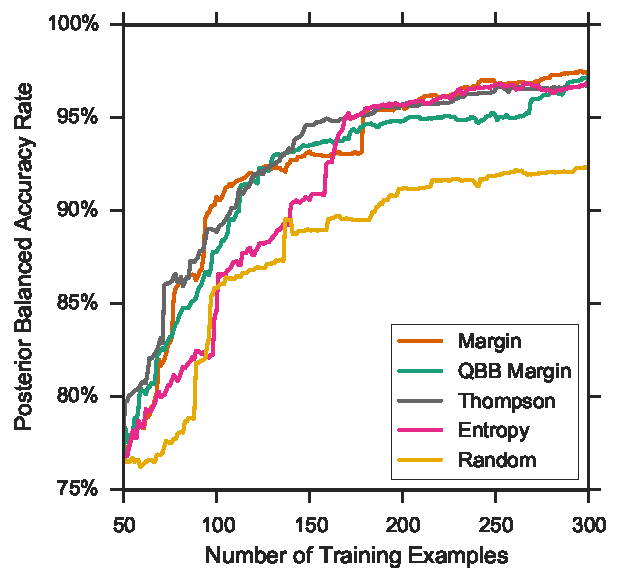
\includegraphics[width=0.99\linewidth]{figures/5_active/vstatlas_ur_ind_upper}
		\caption{Better than random sampling}
		\label{fig:vstatlas_ur_ind_upper}
	\end{subfigure}
	\caption[Learning curves with heuristics (VST ATLAS, unbalanced, logistic)]{
		Learning curves with heuristics (VST ATLAS, unbalanced pool, logistic regression)}
	\label{fig:vstatlas_ur_ind}
\end{figure}

\begin{figure}[p]
	\centering
	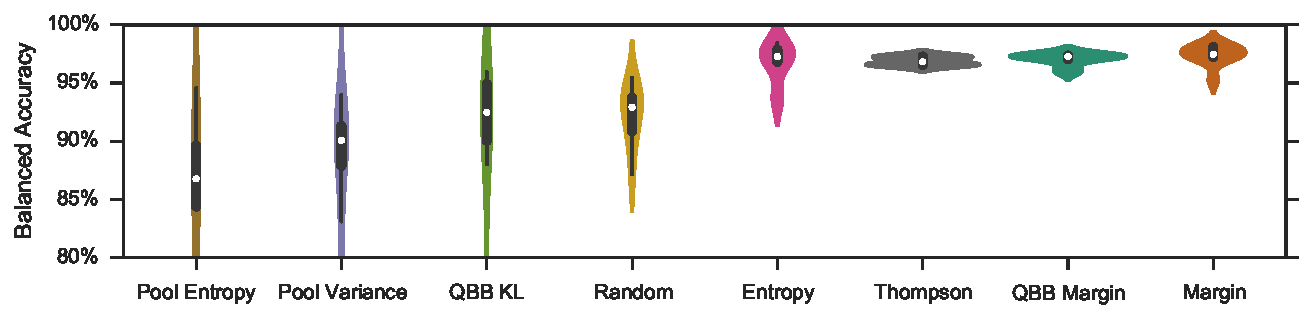
\includegraphics[width=\textwidth]{figures/5_active/vstatlas_ur_ind_violin}
	\caption[Violin plots of final accuracy rates (VST ATLAS, unbalanced, SVM RBF)]{
		Violin plots of final accuracy rates (VST ATLAS, unbalanced pool, SVM RBF)}
	\label{fig:vstatlas_ur_ind_violin}
\end{figure}

\begin{figure}[p]
	\centering
	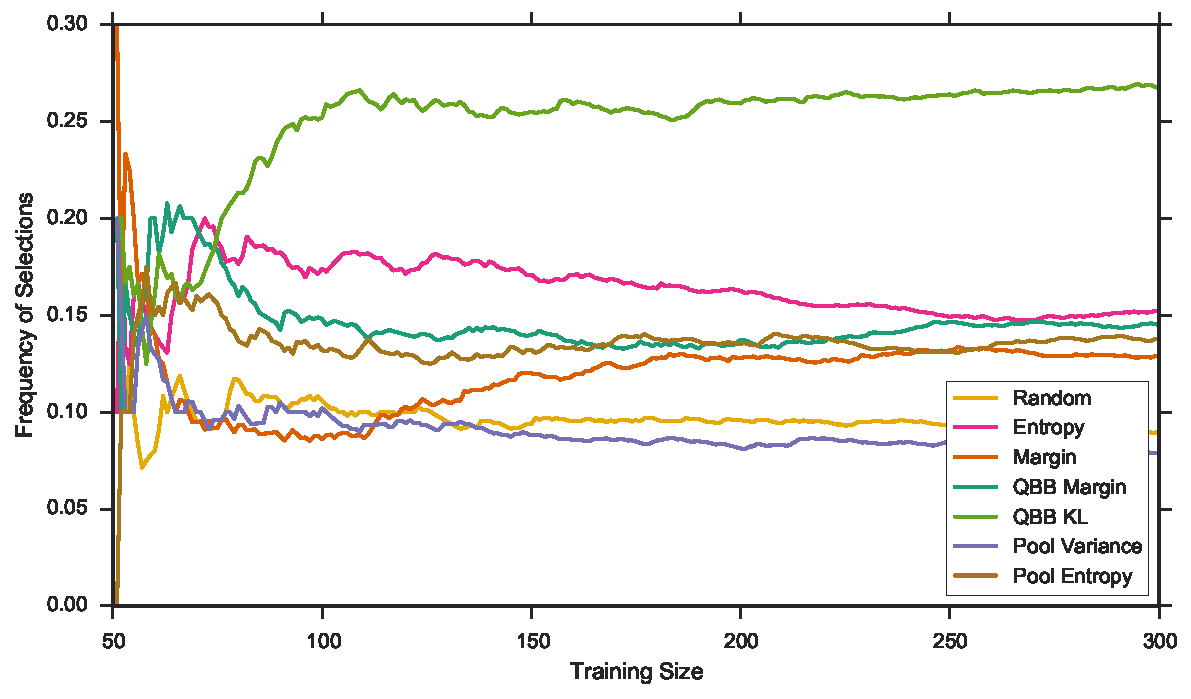
\includegraphics[width=\textwidth]{figures/5_thompson/vstatlas_ur_frequencies}
	\caption[Heuristic selection frequency (VST ATLAS, unbalanced, SVM RBF)]{
		Heuristic selection frequency (VST ATLAS dataset, unbalanced pool, SVM RBF)}
	\label{fig:vstatlas_ur_frequencies}
\end{figure}

\begin{figure}[p]
	\centering
	\begin{subfigure}{.5\textwidth}
		\centering
		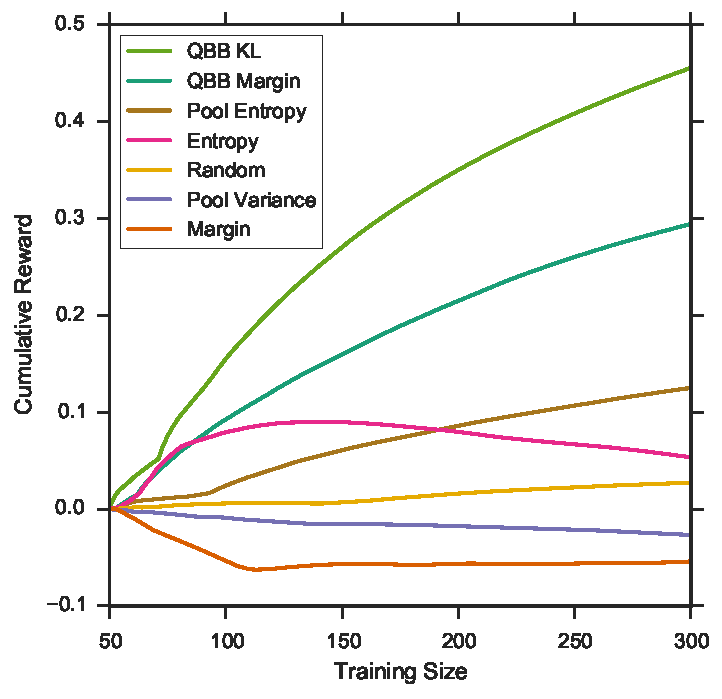
\includegraphics[width=0.99\textwidth]{figures/5_thompson/vstatlas_ur_sum_rewards}
		\caption{Cumulative reward}
		\label{fig:vstatlas_ur_sum_rewards}
	\end{subfigure}%
	\begin{subfigure}{.5\textwidth}
		\centering
		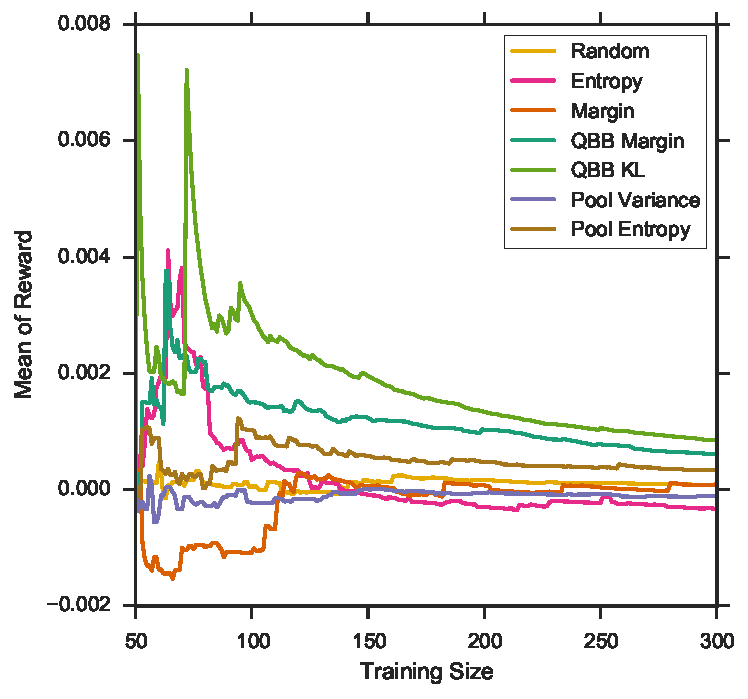
\includegraphics[width=0.99\linewidth]{figures/5_thompson/vstatlas_ur_avg_rewards}
		\caption{Mean of reward}
		\label{fig:vstatlas_ur_avg_rewards}
	\end{subfigure}
	\caption[Reward of heuristics (VST ATLAS, unbalanced, SVM RBF)]{
		Reward of heuristics (VST ATLAS dataset, unbalanced pool, SVM RBF)}
	\label{fig:vstatlas_ur_rewards}
\end{figure}


%%% Local Variables: 
%%% mode: latex
%%% TeX-master: "thesis"
%%% End: 
